\documentclass[a4paper,12pt]{article}
\usepackage[notoc]{HaotianReport}

\title{\SI{10}{\kW}光伏阵列建模及MPPT策略分析}
\author{邓思成,刘昊天}
\authorinfo{电41班, 2014010934, 2014010942}
\runninghead{太阳能光伏发电及其应用2017年最终报告}
\studytime{2017年6月}

\begin{document}
    \begin{abstract}
        简述任务完成情况
        \begin{keywords}
            光伏发电,MPPT,多峰值,光照变化
        \end{keywords}
    \end{abstract}
    \maketitle
    %\newpage
    \section{实验目的} % (fold)
    \label{sec:实验目的}
    \begin{enumerate}[noitemsep, topsep=0pt]
        \item 检验课程学习结果
        \item 增强按目标寻找、归纳、组织知识点的能力
        \item 综合使用光伏发电相关知识
        \item 探索实际前沿问题的控制策略
    \end{enumerate}
    % section 实验目的 (end)
    \section{实验说明} % (fold)
    \label{sec:实验说明}
    任务见任务说明文档。

    在本次实验中,我们采用了MATLAB作为仿真平台,以m文件为基础,对各个任务进行了详尽的分析与解答。
    % section 实验说明 (end)
    \section{任务一} % (fold)
    \label{sec:任务一}
    \paragraph{任务描述} % (fold)
    本任务要求完成如下四点。
    % paragraph 任务描述 (end)
    \begin{enumerate}[noitemsep,topsep=0pt]
    \item 搭建光伏阵列模型,满足给定设置,能依据假定光照合理变化,能用于系统仿真;
    \item 实现 MPPT 控制策略,最经典的扰动观察和电导增量法中的一个即可;
    \item 实现改建的 MPPT 控制策略,可以使用变步长或者功率预测算法,也可以根据文献或者自己的想法给出的新策略;
    \item 对上述任务进行性能分析,包括光伏阵列特性曲线、MPPT 稳态特性、MPPT 暂态特性、改进 MPPT 性能提高对比分析等;
    \end{enumerate}

    \subsection{光伏阵列模型搭建} % (fold)
    \label{sub:光伏阵列模型搭建}
    我们知道,光伏阵列的UI特性可以表达为\cref{eq:iv}所示的公式与\cref{fig:pv}所示的电路。其中,$R_p$是一个并联大电阻,在本任务给定的条件下,其值很大,可以等效为$+\infty$。
    \begin{equation}
        I=I_{ph}-I_0 (\exp{[\frac{q(U+I R_s)}{AKT}}]-1)-\frac{U+I R_s}{R_p}
        \label{eq:iv}
    \end{equation}
    \begin{figure}[htbp]
        \centering
        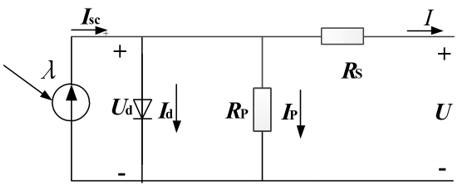
\includegraphics[width=0.65\textwidth]{pv.png}
        \caption{光伏板等效电路}
        \label{fig:pv}
    \end{figure}    
    根据第二次作业中的推导,在给定$I_{sc},U_{oc},I_{mpp},U_{mpp},P_m=U_{mpp}I_{mpp}$的条件后,可以推导出“四参数”模型如\cref{eq:iv4,eq:Io,eq:Rs,eq:Iph,eq:N}所示。

    \begin{equation}
        I=I_{ph}-I_0 (\exp{[\frac{U+I R_s}{N}}]-1)
        \label{eq:iv4}
    \end{equation}
    \begin{equation}\label{eq:Io}
          I_o=\displaystyle\frac{I_{ph}}{e^{CU_{oc}}-1}
    \end{equation}
    \begin{equation}\label{eq:Rs}
          R_s=\displaystyle\frac{1}{I_{mpp}}\left(U_{mpp}-\displaystyle\frac{I_{mpp}}{C\left(I_{ph}+I_o-I_{mpp}\right)}\right)
    \end{equation}
    \begin{equation}\label{eq:Iph}
          I_{ph}\approx I_{sc}
    \end{equation}
    \begin{equation}\label{eq:N}
          N=1/C\approx\displaystyle1/(\frac{1}{2U_{mpp}-U_{oc}}\left(\ln\displaystyle\frac{I_{ph}-I_{mpp}}{I_{ph}}+\displaystyle\frac{I_{mpp}}{I_{ph}-I_{mpp}}\right))
    \end{equation}

    四参数模型中的$I_{ph}$是指在给定的测试条件下的光生电流,此处条件为\SI{1000}{\W\per\meter\squared}的光照强度。光生电流随温度、光照强度的变化情况如\cref{eq:iphlt}所示,其中$\alpha$为一常数。当温度不变时,有\cref{eq:iphlambda}所示的关系。在本任务中,可以以光生电流变化的比例反映光照强度变化的比例。
    \begin{equation}
        I_{ph}=I_{ph0}(1+\alpha \Delta T)\frac{\lambda}{1000}
        \label{eq:iphlt}
    \end{equation}
    \begin{equation}        
        I_{ph} \propto \lambda, T=\text{const}
        \label{eq:iphlambda}
    \end{equation}
    
    在本任务中,逆变器看成一个理想的受控电压源,因此需要从光伏模型的$U$求解$I$。这需要求解一个非线性方程,使用MATLAB自带的fsolve函数求解较慢,因此采用朴素的牛顿迭代法求解,并排除不可行域($I>I_{ph}+I_0$)。这种方式时结果有实际意义,且提升了求解效率。单个光伏模型的代码如\cref{lst:single}所示。
    \lstinputlisting[label=lst:single,language=matlab]{../PvFunctionI.m}
    
    画出标准情况下的PV特性曲线和IV特性曲线,如\cref{fig:bare-pviv}所示。可以看到,其最大功率点、开路电压、短路电流与任务描述一致。TODO:标记最大功率点
    \begin{figure}[htbp]
        \centering
        \includegraphics[width=0.9\textwidth]{../figure/bare-pviv.eps}
        \caption{原始光伏阵列特性曲线}
        \label{fig:bare-pviv}
    \end{figure}

    为了验证模型的正确性,可以令光照在\SIrange{100}{1200}{\W\per\meter\squared}范围内变化,观察其最大功率点的变化情况。可以看到\cref{fig:p-v-many}中,在这个合理的范围内,最大功率点组成的曲线是向右倾斜的,符合经验。TODO:最大功率点连线
    \begin{figure}[htbp]
        \centering
        \includegraphics[width=0.9\textwidth]{../figure/p-v-many.eps}
        \caption{不同光照下的PV曲线}
        \label{fig:p-v-many}
    \end{figure}
    % subsection 光伏阵列模型搭建 (end)
    \subsection{常规MPPT控制策略} % (fold)
    \label{sub:常规mppt控制策略}
    TODO:INC改P\&O

    最常见的MPPT控制策略有两种,即电导增量法INC和扰动观察法P\&O。
    \begin{figure}[htbp]
        \centering
        \includegraphics[width=0.9\textwidth]{../figure/simple-inc.eps}
        \caption{光照恒定条件下成功跟踪}
        \label{fig:simple-inc}
    \end{figure}
    \begin{figure}[htbp]
        \centering
        \includegraphics[width=0.9\textwidth]{../figure/p&o-fault.eps}
        \caption{扰动观察法在光照变化下的跟踪情况}
        \label{fig:po-fault}
    \end{figure}
    \begin{figure}[htbp]
        \centering
        \includegraphics[width=0.9\textwidth]{../figure/p&o-upt-fault.eps}
        \caption{扰动观察法在光照变化下的电压、功率情况}
        \label{fig:po-fault-upt}
    \end{figure}
    % subsection 常规mppt控制策略 (end)
    \subsection{改进MPPT:功率预测法} % (fold)
    \label{sub:改进mppt_功率预测法}
    \begin{figure}[htbp]
        \centering
        \includegraphics[width=0.9\textwidth]{../figure/p&o.eps}
        \caption{功率预测法在光照变化下的跟踪情况}
        \label{fig:po}
    \end{figure}
    \begin{figure}[htbp]
        \centering
        \includegraphics[width=0.9\textwidth]{../figure/p&o-upt.eps}
        \caption{功率预测法在光照变化下电压、功率情况}
        \label{fig:po-upt}
    \end{figure}
    % subsection 改进mppt_功率预测法 (end)
    \subsection{算法性能分析} % (fold)
    \label{sub:算法性能分析}
    
    % subsection 算法性能分析 (end)
    % section 任务一 (end)
    \section{任务二} % (fold)
    \label{sec:任务二}
    \paragraph{任务描述} % (fold)
    本任务要求完成如下三点。
    % paragraph 任务描述 (end)
    \begin{enumerate}[noitemsep,topsep=0pt]
    \item 将任务一中的光伏阵列分拆成具有串并联结构的几个子阵列,光照均匀时,总阵列的输出特性与任务一中的光伏阵列相同,合理设置子阵列的光照参数,使总阵列输出的 P-V 特性曲线上有两个(包含两个)以上的局域最大功率点,并且全局最大功率点电压和开路电压之间存在至少一个局域最大功率点,实现该光伏阵列模型。
    \item 保持光照不变,实现多峰值光伏阵列上的常规 MPPT 控制策略仿真和分析。
    \item 保持光照不变,尝试能够应对多峰值光伏阵列的新型 MPPT 控制策略,并给出分析。
    \end{enumerate}    
    \subsection{多峰值光伏阵列} % (fold)
    \label{sub:多峰值光伏阵列}
    \begin{figure}[htbp]
        \centering
        \includegraphics[width=0.9\textwidth]{../figure/curve-multimax.eps}
        \caption{多峰值光伏曲线}
        \label{fig:curve-multimax}
    \end{figure}
    \begin{figure}[htbp]
        \centering
        \includegraphics[width=0.9\textwidth]{../figure/curve-singlemax.eps}
        \caption{均匀光照下的串并联阵列特性曲线}
        \label{fig:curve-singlemax}
    \end{figure}
    % subsection 多峰值光伏阵列 (end)
    \subsection{常规MPPT策略在多峰值情况下的应用} % (fold)
    \label{sub:常规mppt策略在多峰值情况下的应用}
    \begin{figure}[htbp]
        \centering
        \includegraphics[width=0.9\textwidth]{../figure/mppt-fail-pv.eps}
        \caption{多峰值下常规MPPT策略的跟踪轨迹}
        \label{fig:mppt-fail-pv}
    \end{figure}
    \begin{figure}[htbp]
        \centering
        \includegraphics[width=0.9\textwidth]{../figure/mppt-fail-upt.eps}
        \caption{多峰值下常规MPPT策略的电压、功率情况}
        \label{fig:mppt-fail-upt}
    \end{figure}
    % subsection 常规mppt策略在多峰值情况下的应用 (end)
    \subsection{改进MPPT策略:改良的粒子群算法} % (fold)
    \label{sub:改进mppt策略_改良的粒子群算法}
    \begin{figure}[htbp]
        \centering
        \includegraphics[width=0.9\textwidth]{../figure/p-v-one.eps}
        \caption{标幺功率、标幺电压关系曲线}
        \label{fig:p-v-one}
    \end{figure}
    \begin{figure}[htbp]
        \centering
        \includegraphics[width=0.9\textwidth]{../figure/umpp-iph-one.eps}
        \caption{最大功率点标幺电压随光照变化情况}
        \label{fig:umpp-iph-one}
    \end{figure}
    \begin{figure}[htbp]
        \centering
        \includegraphics[width=0.9\textwidth]{../figure/mppt-pv.eps}
        \caption{改良算法的跟踪轨迹}
        \label{fig:mppt-pv}
    \end{figure}
    \begin{figure}[htbp]
        \centering
        \includegraphics[width=0.9\textwidth]{../figure/mppt-upt.eps}
        \caption{改良算法的电压、功率变化情况}
        \label{fig:mppt-upt}
    \end{figure}
    % subsection 改进mppt策略_改良的粒子群算法 (end)
    % section 任务二 (end)
    \begin{appendix}
        \section{分工情况} % (fold)
        \label{sec:fengong}
        \paragraph{邓思成} % (fold)
        \label{par:邓思成}
        部分模型代码;部分MPPT代码;部分报告;部分PPT;

        总体工作量:50\%。
        % paragraph 邓思成 (end)
        \paragraph{刘昊天} % (fold)
        \label{par:刘昊天}
        部分模型代码;部分MPPT代码;部分报告;部分PPT;

        总体工作量:50\%。
        % paragraph 刘昊天 (end)
    \end{appendix}
\iffalse
\begin{itemize}[noitemsep,topsep=0pt]
%no white space
\end{itemize}
\begin{enumerate}[label=\Roman{*}.,noitemsep,topsep=0pt]
%use upper case roman
\end{enumerate}
\begin{multicols}{2}
%two columns
\end{multicols}
\fi
\end{document}